\section{Comparison with hfbcs-qrpa code}
All the calculations are carried out using SLy5 parameters.
\begin{align}
  \expval{r^2_{p}} = \frac 1 Z \int r^2 \rho_p(\mathbf r) d^3 \mathbf r\\
  \expval{r^2_{n}} = \frac 1 N \int r^2 \rho_n(\mathbf r) d^3 \mathbf r\\
  \expval{r^2_{ch}} = \expval{r^2_{p}} + \expval{r^2}_P + \expval{r^2}_N + \frac 1 Z \bigg(\frac \hbar {mc}\bigg{)}^2\sum_\alpha \mu_{\tau_\alpha}\expval{\boldsymbol{\sigma}\cdot \boldsymbol \ell }_\alpha
\end{align}
\begin{table}[ht]
  \centering
  \caption{$^{16}$O Including spin-gradient terms, spin-orbit interaction, and Coulomb field}
  \label{tab:confronto}
  \begin{tabular}{lrccc}
    \multicolumn{5}{c}{\textbf{Physical quantities}}\\
    \addlinespace[0.3em]
    \midrule
    && GCG & hfbcs\_qrpa & $\Delta\%$ \\
    \midrule
    $E_{\text{TOT}}$& [MeV] & -128.424 & -128.400 & \num{1.87e-2} \\
    $\expval{ r^2_n}^{1/2}$ &[fm] & 2.6581 & 2.6585 & \num{1.50e-2}\\
    $\expval{ r^2_p}^{1/2}$ &[fm] & 2.6832 & 2.6836 & \num{1.49e-2}\\
    $\expval{ r^2_{ch}}^{1/2}$ &[fm] & 2.7806 & 2.7803 & \num{1.08e-2}\\
    \midrule
    \addlinespace[1.3em]
    \multicolumn{5}{c}{\textbf{Neutron energy levels}}\\
    \addlinespace[0.3em]
    \midrule
    && GCG & hfbcs\_qrpa & $\Delta\%$ \\
    \midrule
    1s$_{1/2}$ &[MeV] & -36.142 & -36.137 & \num{1.38e-2}\\
    1p$_{3/2}$ &[MeV] & -20.613 & -20.611 & \num{9.70e-3}\\
    1p$_{1/2}$ &[MeV] & -14.426 & -14.428 & \num{1.38e-2}\\
    \midrule
    \addlinespace[1.3em]
    \multicolumn{5}{c}{\textbf{Proton energy levels}}\\
    \addlinespace[0.3em]
    \midrule
    && GCG & hfbcs\_qrpa & $\Delta\%$ \\
    \midrule
    1s$_{1/2}$ &[MeV] & -32.349 & -32.345 & \num{1.23e-2}\\
    1p$_{3/2}$ &[MeV] & -17.139 & -17.137 & \num{1.16e-2}\\
    1p$_{1/2}$ &[MeV] & -11.081 & -11.082 & \num{9.02e-3}\\
    \bottomrule
  \end{tabular}
\end{table}
\begin{figure}
  \centering
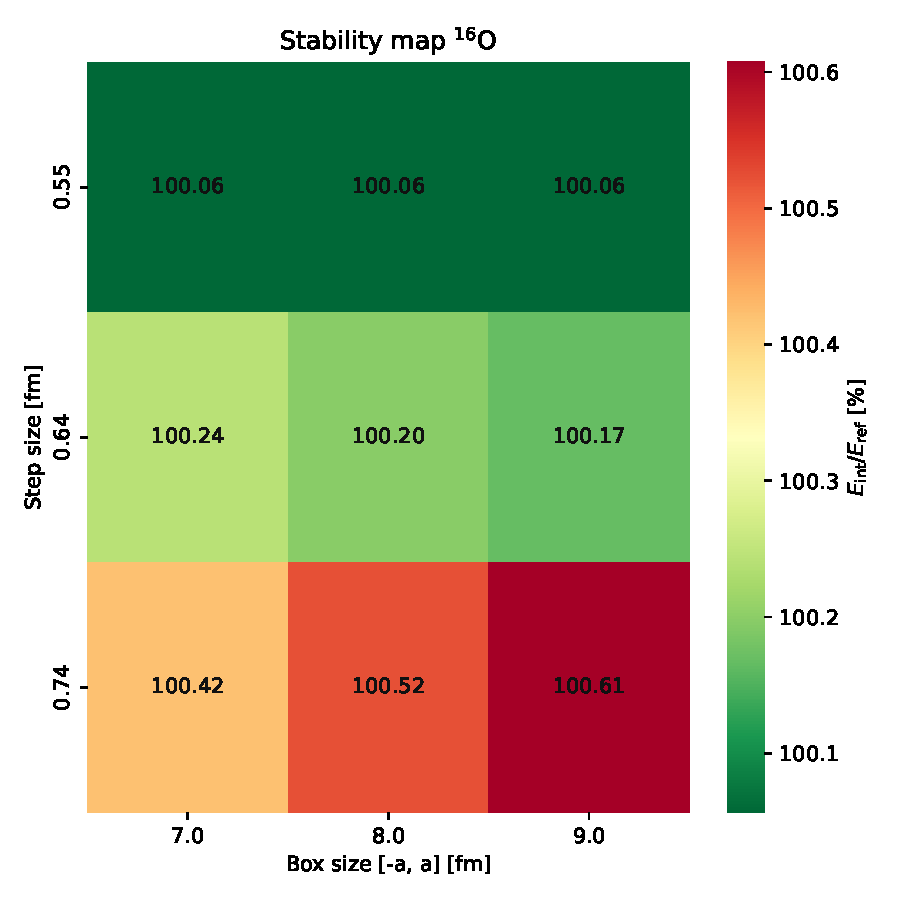
\includegraphics[width = 0.8\textwidth, keepaspectratio]{figures/stability.pdf}
\caption{Stability heatmap for unconstrained GCG against hfbcs\_qrpa reference value}
\end{figure}

